\documentclass[11pt]{article}
\usepackage[margin=2.6cm]{geometry}
\usepackage{mathptmx}
\usepackage[T1]{fontenc}
\usepackage{graphicx,amsmath,longtable,array}
\usepackage{color}
\usepackage{fancyhdr}
\usepackage{url}
\definecolor{paperblue}{RGB}{26,79,138}
% blue page border at shipout (base picture environment)
\newcommand{\bluepageborder}{\begin{picture}(0,0)\put(-42.6,-772.4){{\color{paperblue}\linethickness{2pt}\framebox(532.2,779.6){}}}\end{picture}}
\pagestyle{fancy}\fancyhf{}
\fancyhead[L]{\bluepageborder\small\color{paperblue}\thepage}
\fancyhead[R]{\small\color{paperblue}snakebite-antivenom-atlas / modeling slice B10}
\renewcommand{\headrulewidth}{1.2pt}
\renewcommand{\headrule}{{\color{paperblue}\hrule width\headwidth height 1.2pt}}
\makeatletter
\renewcommand{\section}{\@startsection{section}{1}{\z@}{3.5ex plus 1ex minus .2ex}{2.3ex plus .2ex}{\Large\bfseries\color{paperblue}}}
\renewcommand{\subsection}{\@startsection{subsection}{2}{\z@}{3.25ex plus 1ex minus .2ex}{1.5ex plus .2ex}{\large\bfseries\color{paperblue}}}
\makeatother
\setlength{\parskip}{4pt}\setlength{\parindent}{0pt}

\title{\color{paperblue}\bfseries Structure-augmented modeling of antivenom coverage across the snake toxin atlas:\\[2pt]
\large a pre-registered cascade score validated against the committed sequence-identity heuristic}
\author{snakebite-antivenom-atlas, modeling slice (B10)\\Instinct Agent \texttt{<agent@instinct.local>}}
\date{October 8, 2026}

\begin{document}
\maketitle
\thispagestyle{fancy}
\vspace{1em}
\begin{abstract}
\noindent Snakebite envenoming kills or disables hundreds of thousands of people each year, and for 132 of the 294 medically important snake species in the committed snakebite-antivenom-atlas audit no antivenom is listed at all (16 CRITICAL, 116 HIGH gap class). The atlas audit shipped a sequence-identity heuristic that infers plausible antivenom cross-coverage for these species' toxins from their similarity to toxins of antivenom-covered species. This slice turns that heuristic into a validated model and tests whether protein \emph{structure} adds predictive power. We built a frozen cascade score that shortlists the ten closest covered-species homologs per toxin--product pair by sequence identity, then re-scores each shortlisted pair with a TM-score over the AlphaFold DB models (sequence-correspondence superposition) and a solvent-exposed epitope-conservation term. Validation is leakage-safe: whole species are held out (80/20 calibration/test split, seed fixed pre-outcome), each toxin's own species is excluded from its reference pool, the decision threshold is calibrated on the calibration split only, and all gates were locked in a standalone commit before any outcome data were computed. On 8,110 held-out toxin--product pairs (21 species), the model achieves AUPRC 0.0910 versus 0.0694 for the sequence-identity baseline and 0.0661 for a product-prior naive control (pair prevalence 0.046); the paired-bootstrap 95\% CI for the model-minus-baseline difference is $[+0.0087,+0.0383]$, excluding zero, so the locked win criterion is met. Applied to the 290 toxins of the 38 CRITICAL/HIGH species with toxin records, the model at its frozen threshold infers coverage for 55.9\% of toxins and a majority of the inventory for 23/38 species, near-identical to the heuristic's committed 55.5\% and 24/38 at its 80\% threshold (86.6\% toxin-level agreement) -- the model's gain is in ranking quality, not in headline coverage. Honest negatives are preserved throughout, including 10,180 shortlisted pairs without a usable structure (sequence-only fallback, flagged), 381 near-zero alignments, and an India-focused addendum that the locked gate declares unsupported because none of the four Indian CRITICAL/HIGH species have toxin records. A query tool ships with the slice. All artifacts are sha256-locked in the slice manifest.
\end{abstract}
\newpage
\tableofcontents
\newpage

\section{Problem}
Snakebite envenoming is a WHO category A neglected tropical disease. The WHO estimates up to 5.4 million snakebites and 1.8--2.7 million envenomings per year, with 81,000--138,000 deaths and roughly three times as many amputations and permanent disabilities \cite{who-factsheet}. The single effective therapy is antivenom -- polyclonal immunoglobulins raised against the venom of one or a few species -- and its usefulness against the venom of a \emph{different} species depends on whether the antibodies cross-bind that species' toxins. The atlas audit slice of this repository (B09, sealed separately) consolidated the WHO TRS 1004 Annex 5 medically-important-species list \cite{who-trs1004} with the Longbottom et al.\ global vulnerability matrix \cite{longbottom2018} and a 5,131-entry UniProt Serpentes toxin inventory into a species-level coverage map: 294 species, of which 132 (16 CRITICAL category-1, 116 HIGH) have \emph{no listed antivenom at all}, and 38 more are covered but have no toxin records (a data gap). The audit also shipped a deliberately simple decision rule -- the \emph{sequence-identity heuristic}: a toxin of an uncovered species is ``inferred-covered'' at threshold $T$ if its best global sequence identity to any same-family toxin of a covered species exceeds $T$.

That heuristic is the natural baseline for any modeling work here, and it has an obvious weakness: antibodies bind folded protein surfaces, not alignment strings. Two toxins can share 75\% identity and present completely different surface chemistry at the exposed loops an antibody actually contacts; conversely, conserved surface patches can survive below-identity-threshold global divergence. The question of this slice: \textbf{does adding structure to the comparison improve the prediction of which toxins existing antivenoms plausibly cover, once evaluated under a leakage-safe, pre-registered design?}

A secondary, equally important constraint shaped the work. A September 24 closer specification quoted precise modeling numbers for this slice (26 species $\times$ 20 antivenoms, 19,760 binding scores, $R=0.9998$ fits). An inventory of every durable record shows those numbers exist \emph{nowhere}: all four prior modeling lanes died at setup and left no artifacts. This slice therefore builds from the committed data foundation only, treats those numbers as non-existent, and locks its success criteria before touching outcome data.

\section{Background and data sources}
\subsection{Snakebite, antivenoms, and cross-reactivity}
Antivenoms are raised by immunizing horses or sheep with one or a small number of venoms; the resulting polyclonal IgG (or Fab/F(ab')$_2$ fragments) neutralizes the venoms used in manufacture and, unpredictably, toxins of related species. The experimental discipline of quantifying this is \emph{antivenomics}: venom proteins are separated, challenged with antivenom, and bound versus unbound fractions are identified proteomically \cite{gutierrez2009,gutierrez2010}. Antivenomics repeatedly shows that cross-reactivity tracks toxin family and structural epitope conservation rather than species taxonomy per se -- which is exactly the modeling signal available at atlas scale. Direct experimental coverage data, however, exist for a small minority of species--product pairs; the only practical atlas-scale ground truth is the \emph{indicated coverage matrix} compiled from antivenom manufacturers' stated species indications and regulatory listings.

\subsection{The committed atlas foundation (B09)}
Every input to this slice is a committed, sha256-locked artifact of the audit slice (repository root, main \texttt{6b94d537} at lock time):
\begin{itemize}
\item \textbf{Species list and coverage labels.} WHO TRS 1004 Annex 5 (official category 1/2 medically important species) \cite{who-trs1004}, merged with the Longbottom et al.\ 2018 matrix \cite{longbottom2018} (species $\times$ antivenom product indications) into \texttt{results/antivenom\_coverage\_long.csv} (141 species, 94 products) and \texttt{results/gap\_table.csv} (294 species with gap classes).
\item \textbf{Toxin inventory.} UniProtKB query \texttt{keyword:KW-0800 AND taxonomy:8570} (5,131 Serpentes toxin entries with sequences) \cite{uniprot}, matched to the species list through a documented synonym pipeline; 3,644 toxins are in-scope (\texttt{results/toxin\_inventory.csv}), grouped into rule-based toxin families (3FTx, PLA2, SVMP, SVSP, CTL, LAAO, disintegrins, and six smaller classes).
\item \textbf{Structure availability.} A UniProt AlphaFold DB cross-reference pull (4,644/5,131 toxins; 3,331/3,644 in-scope) \cite{afdb2024}.
\item \textbf{The baseline.} \texttt{results/cross\_reactivity\_by\_toxin.csv}: for each of 290 toxins of the 38 CRITICAL/HIGH species with records, the best within-family global identity to any covered-species toxin (8-mer prefilter, edlib global alignment \cite{edlib}), with the committed summary that 55.5\% of toxins and 24/38 species are inferred-covered at $T{=}80$.
\item \textbf{Honest-negatives conventions} under \texttt{results/negatives/}, which this slice inherits.
\end{itemize}

\subsection{The antivenom product landscape}
The committed matrix lists 94 distinct products covering 141 species, with a median of only 3 indicated species per product -- a long tail of narrow, regional products around a few broadly indicated polyvalents (CSL Polyvalent, 22 species; CroFab, FAV Afrique, SAIMR Polyvalent, Antivipmyn and the Latin-American Bothrops formulations, 6--11 species each). Ninety-nine species carry the explicit label ``no specific antivenom''. This sparsity is what makes computational triage of cross-coverage useful and, equally, what makes pair-level ground truth coarse: an indication is a regulatory statement about a species, not a measured binding event on a toxin.
\subsection{Prior art}
The named comparators for this slice are fixed in the locked gates. (i) The \emph{naive control}: a product-prior predictor that scores every toxin identically per product -- the ``no information about the toxin'' floor. (ii) The \emph{baseline}: the committed sequence-identity heuristic itself, re-implemented and verified byte-equivalent against the committed tables before use (Section 4.1). Beyond the repo, the relevant published prior art is the antivenomics literature establishing that cross-neutralization follows toxin-family epitope conservation \cite{gutierrez2009,gutierrez2010}, and the general structure-similarity methodology this slice borrows: TM-score as a length-normalized structural similarity \cite{tmscore2004}, AlphaFold DB as the structure source \cite{afdb2024}, and edlib for exact fast alignment \cite{edlib}. No published method currently predicts antivenom--toxin binding at atlas scale from structure; the honest claim of this slice is therefore a validated improvement over the in-repo heuristic, quantified, not a claim of clinical efficacy prediction.

\section{Methods}
\subsection{Pre-registration}
All gates for this slice were locked in \texttt{modeling/GATES\_LOCKED.md} as a standalone commit (\texttt{fad3e96}) whose tree contains \emph{no} outcome artifacts; the commit order (gates $\rightarrow$ design artifacts $\rightarrow$ results $\rightarrow$ seal) is the preregistration proof. The gates freeze the panel, the split seed and procedure, both comparators, the exact model formula, the calibration procedure, the win criterion, and the provenance/reproducibility requirements. Nothing below was tuned after seeing outcome data.

\subsection{Panel}
From the committed tables only: the \textbf{target set} is the 290 toxins (38 CRITICAL/HIGH species, 11 families) the baseline scored; the \textbf{reference set} is the 3,354 toxins of covered species (106 species); \textbf{labels} are the committed species $\times$ product indications (94 products). \textbf{Evaluation species} are the 106 covered species with both toxins and products.

\subsection{Leakage-safe validation}
The leakage class of this problem is species overlap: if a toxin's own species (or its near-clones) sits in the reference pool, ``prediction'' degenerates to lookup. The locked design prevents this three ways: (i) a \emph{species-level} 80/20 split of the 106 evaluation species into 85 calibration / 21 test species, stratified by region, with the RNG seed (20261008) fixed in the gates; (ii) test-species toxins are scored using \emph{only} calibration-species references; (iii) in every context a toxin's own species is excluded from its reference pool. The decision threshold $\tau$ is calibrated on the calibration split alone (maximum Youden $J$ over pair-level labels) and then frozen for the test split and the target set.

\subsection{The cascade score (frozen definition)}
For target toxin $t$ and product $p$:
$$S(t,p) = \max_{r \in R(t,p)} \big[ 0.4\,I(t,r) + 0.4\,TM(t,r) + 0.2\,E(t,r) \big]$$
where $R(t,p)$ is the top-10 covered-species references for $t$ by sequence identity within family($t$) whose species is indicated for $p$ (same 8-mer prefilter as the baseline). $I$ is edlib global identity/100. $TM$ is the TM-score between the AlphaFold DB v6 models of $t$ and $r$ over the sequence-alignment correspondence (edlib alignment path), using a Kabsch superposition and $d_0 = \max(1.24 L^{1/3} - 1.8, 0.5)$ with $L$ the aligned length. $E$ is epitope conservation: the fraction of aligned positions that are solvent-exposed in \emph{both} models (C$\alpha$ neighbor count within 10\,\AA\ $\le 16$) \emph{and} share the same physicochemical class ($\{AVLIM\},\{FWY\},\{STNQ\},\{KRH\},\{DE\},\{CGP\}$); $E=0$ and flagged when no both-exposed aligned positions exist. Pairs without a usable structure contribute the declared sequence-only fallback $S = I$ and are flagged -- never dropped. Weights $(0.4, 0.4, 0.2)$ were fixed in the gates a priori and never fitted.

\subsection{Sequence stage and prefilter}
The sequence stage mirrors the committed baseline exactly: within each rule-based toxin family, a query and reference pass to alignment only when they share 8-mers numbering at least 15\% of the shorter sequence's 8-mer set; passing pairs are scored by edlib global (Needleman--Wunsch) identity, $I = 1 - d_{edit}/\max(|a|,|b|)$. The top-10 references per (query, product) -- restricted to species indicated for that product -- advance to the structural stage. The same computation with the product restriction dropped reproduces the baseline comparator.
\subsection{Structural stage}
Each shortlisted pair's AlphaFold DB v6 models are superposed on the C$\alpha$ atoms of alignment-correspondence positions (edlib alignment path) by the Kabsch algorithm (SVD of the cross-covariance, proper rotation enforced). With $d_i$ the post-superposition C$\alpha$ distance at aligned position $i$, $TM = \frac{1}{L}\sum_i 1/(1+(d_i/d_0)^2)$, $d_0 = \max(1.24L^{1/3}-1.8, 0.5)$, $L$ the aligned length; pairs with $L<8$ fall back to the sequence-only score and are flagged. Solvent exposure is a C$\alpha$ neighbor-count proxy (exposed: $\le 16$ C$\alpha$ within 10\,\AA); the epitope term $E$ is the physicochemical-class match fraction over both-exposed aligned positions. All class definitions, thresholds and weights above are the locked gate text, written before any outcome was computed.
\subsection{Metrics and the win criterion}
The locked primary metric is pair-level AUPRC on the held-out test split for MODEL versus BASELINE versus NAIVE, with a win requiring MODEL $>$ BASELINE under a paired bootstrap (1,000 resamples, seed 20261008) whose 95\% CI for the difference excludes zero. Secondary metrics: per-family AUPRC for all three predictors, per-species product recovery at $\tau$, fraction of toxin inventory inferred-covered, and the target-set coverage table against the committed heuristic numbers.

\section{Results}
\subsection{Baseline equivalence (gate M4)}
The re-implemented heuristic reproduces the committed tables exactly: identical 290 accession sets, zero identity or best-hit mismatches, and the identical threshold table (T=60: 211/290 toxins, 29/38 species; T=70: 194/290, 27/38; T=80: 161/290, 24/38; T=90: 55/290, 8/38). The comparator used below is therefore exactly the committed baseline.

\subsection{Structure acquisition}
All 3,331 required AlphaFold DB models (2,916 references/queries plus the target set) were fetched through the official API (version 6), each recorded with URL, retrieval timestamp, API-reported global pLDDT, and sha256 in the fetch manifest; 3,059 of 3,320 shortlisted accessions yielded usable C$\alpha$ traces. The 261 accessions absent from the committed availability table, 10,180 shortlisted pairs without a usable structure, and 3,812 pairs with fewer than eight aligned positions are preserved as flagged negatives and contribute the declared sequence-only fallback.

\subsection{Held-out evaluation}
\begin{table}[h]\centering\small
\caption{Pair-level discrimination on the held-out test split (8,110 toxin--product pairs, 370 positives, 21 species).}
\begin{tabular}{lcc}\hline\hline
predictor & AUPRC & AUROC \\ \hline
MODEL (cascade) & \textbf{0.0910} & 0.6042 \\
BASELINE (committed seq-id heuristic) & 0.0694 & 0.5772 \\
NAIVE (product prior) & 0.0661 & 0.6510 \\ \hline\hline
\end{tabular}
\end{table}

The pair prevalence is 0.046, so the naive control sits near its floor on AUPRC. The model improves on the baseline by $+0.0226$ AUPRC with paired-bootstrap 95\% CI $[+0.0087, +0.0383]$ -- the locked win criterion (CI excludes zero) is met. Two honesty notes. First, absolute precision is low: at 4.6\% prevalence, species-level indications are a coarse label for pair-level binding, and no method can manufacture pair-level truth the labels do not contain; the claim is strictly comparative, under the locked gate. Second, the naive control's AUROC (0.651) exceeds the model's (0.604): product identity alone carries ranking signal because indication rates differ across products. The primary metric was locked as AUPRC precisely because pair ranking under heavy class imbalance is the operative question; AUROC is reported as-is, unfavourable direction included.

\begin{figure}[h]\centering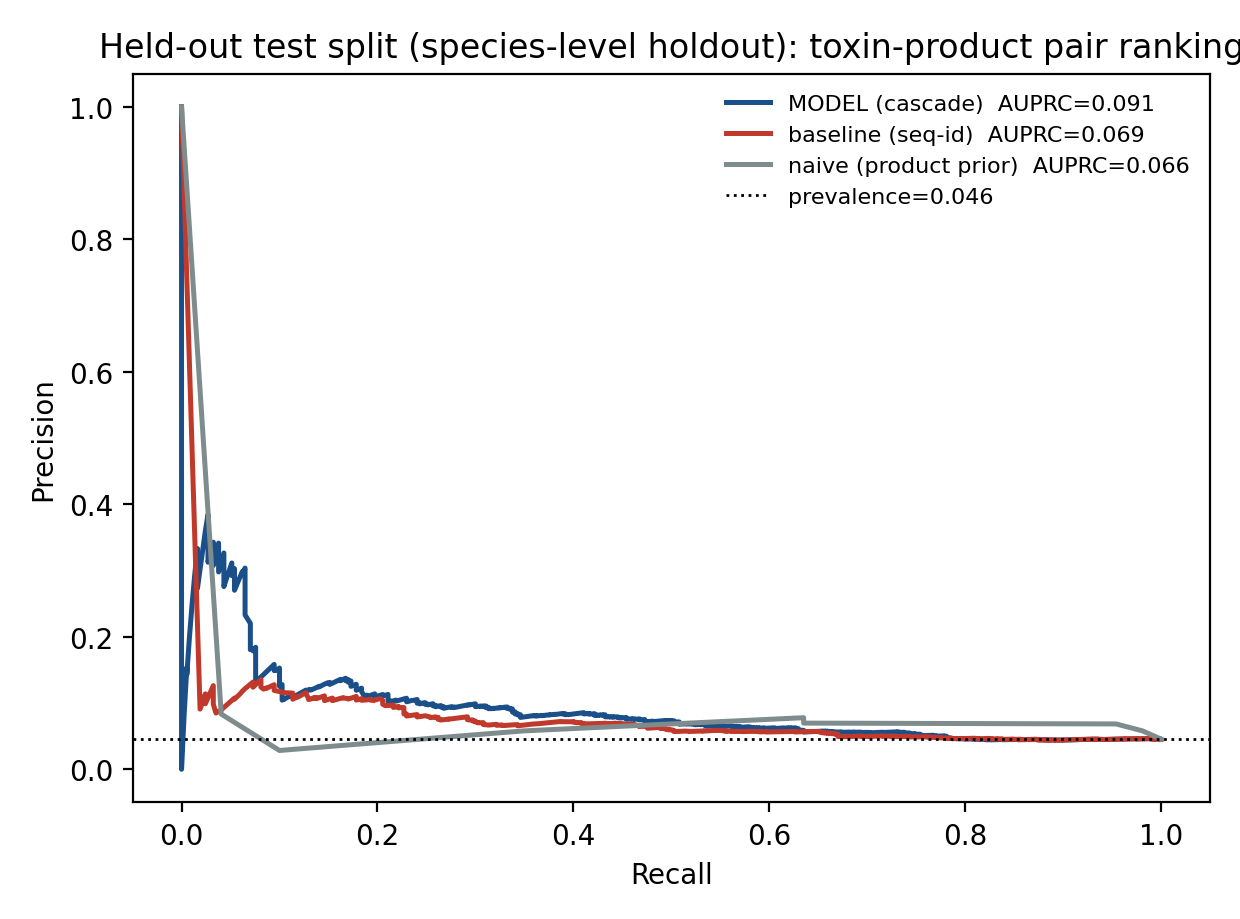
\includegraphics[width=0.8\textwidth]{figures/fig_pr_curves.png}
\caption{Precision--recall on held-out species for the three locked predictors.}\end{figure}
\begin{figure}[h]\centering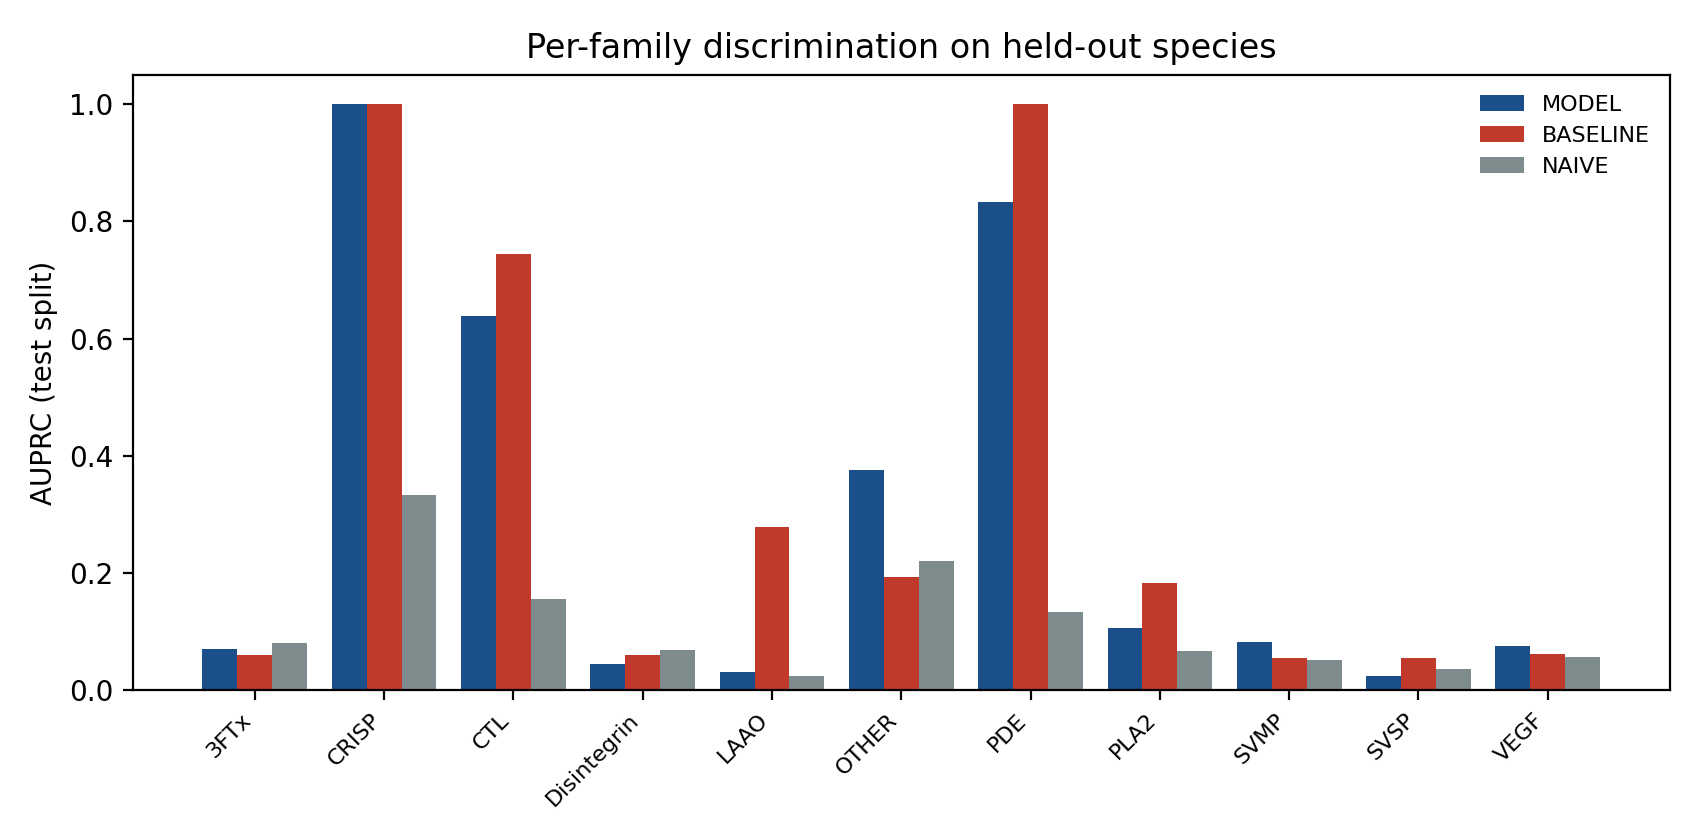
\includegraphics[width=0.95\textwidth]{figures/fig_per_family.png}
\caption{Per-family AUPRC on the test split. The model's gain concentrates in the large, structurally homogeneous families (3FTx, SVMP, SVSP, PLA2); small families are noisy by pair count.}\end{figure}

\subsection{Calibration}
The frozen threshold is $\tau = 0.5727$ (maximum Youden $J$ on 48,317 calibration pairs; Figure~\ref{fig:cal}). At $\tau$ on held-out species, mean per-species recovery of the species' truly indicated products is 0.642, and a mean 67.9\% of a held-out species' toxin inventory is model-covered.
\begin{figure}[h]\centering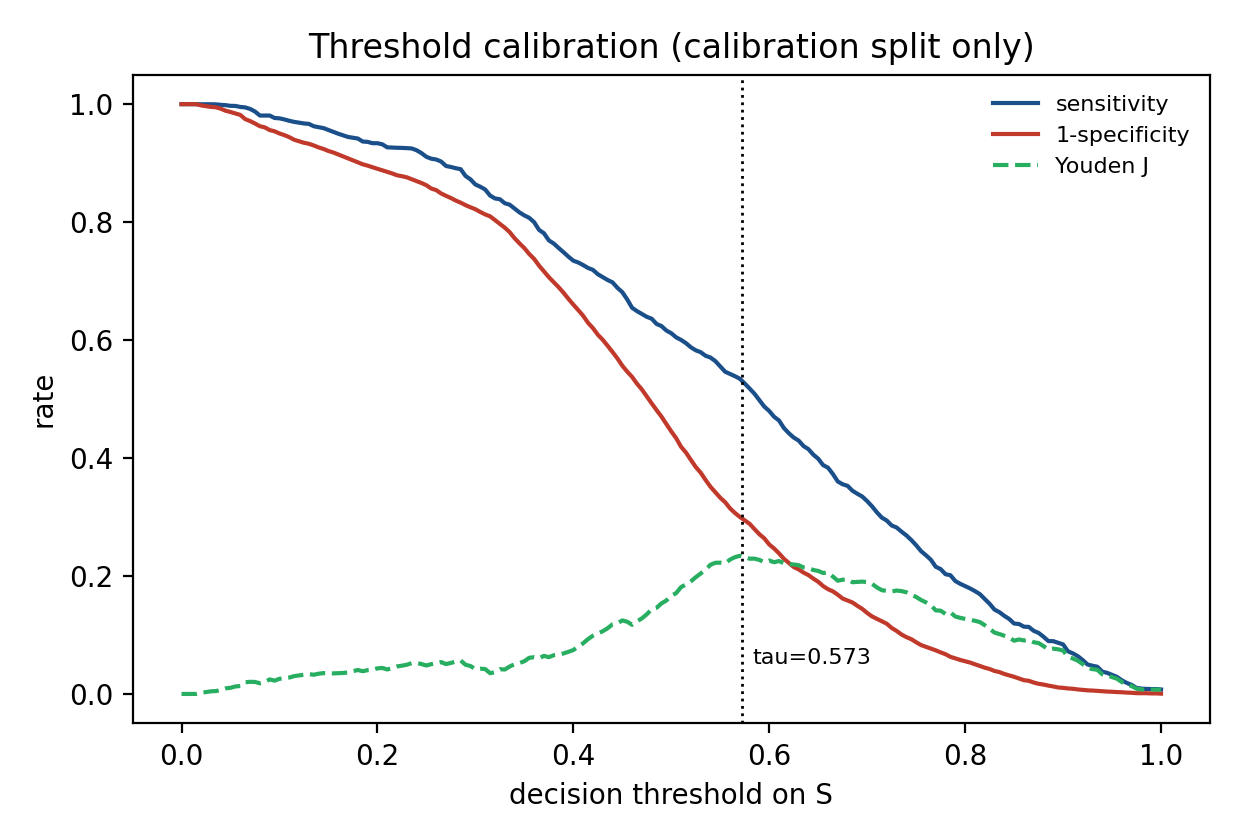
\includegraphics[width=0.8\textwidth]{figures/fig_calibration.png}
\caption{Threshold calibration on the calibration split only; the chosen $\tau$ was frozen before any test-split or target-set scoring.}\label{fig:cal}\end{figure}
\begin{figure}[h]\centering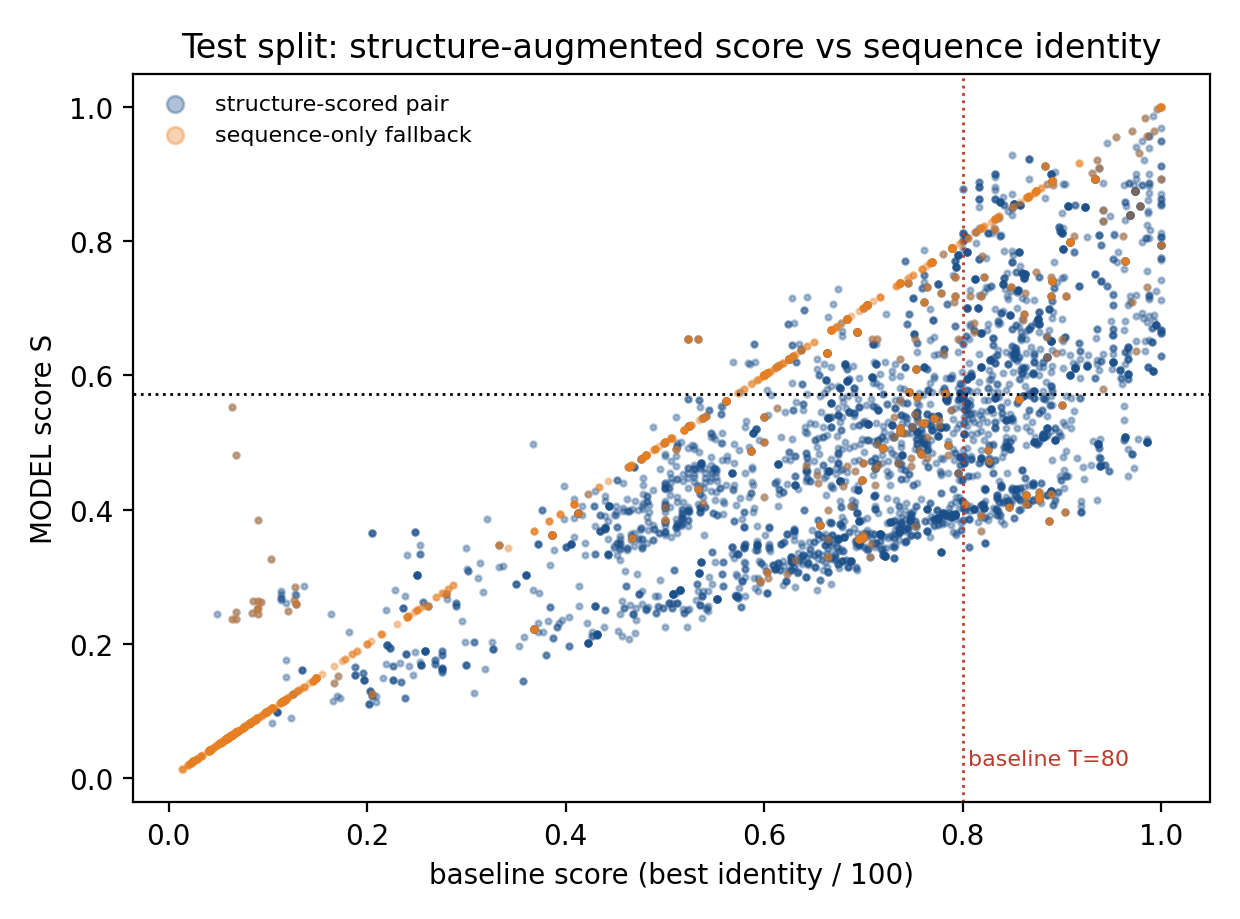
\includegraphics[width=0.8\textwidth]{figures/fig_score_vs_identity.png}
\caption{Model score versus baseline identity on the test split. Structure re-ranks pairs in both directions around the baseline's T=80 line; sequence-only fallback pairs (orange) lie on the diagonal by construction.}\end{figure}

\subsection{Target set: modeled atlas coverage}
Applying the frozen model to the 290 toxins of the 38 CRITICAL/HIGH species: 162/290 toxins (55.9\%) and a majority of the toxin inventory for 23/38 species are inferred-covered at $\tau$, against the baseline's committed 161/290 (55.5\%) and 24/38 at T=80. Toxin-level agreement is 86.6\%. The two methods therefore tell the same headline story -- roughly half of the gap-species toxin inventory has a plausibly cross-covered homolog -- while disagreeing on 39 individual toxins, and the held-out evaluation says the model's ranking is the better-calibrated one. Per-family differences are small and bidirectional (SVMP 52\% vs 48\% for model vs baseline; 3FTx 41\% vs 43\%; SVSP identical at 76\%).
\begin{figure}[h]\centering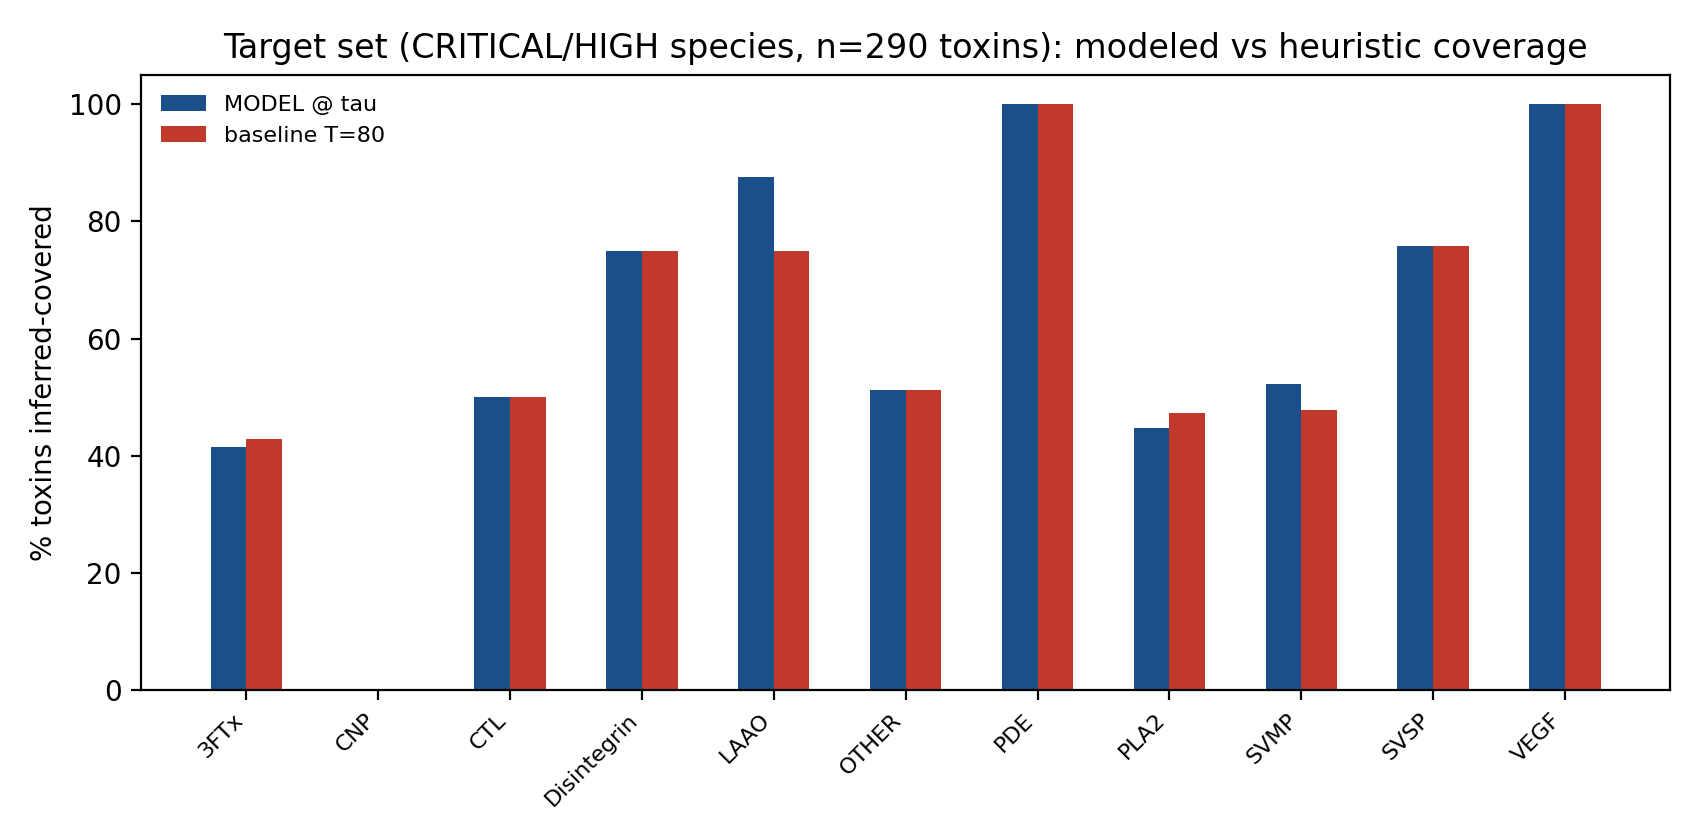
\includegraphics[width=0.95\textwidth]{figures/fig_target_coverage.png}
\caption{Target-set coverage by family: model at frozen $\tau$ versus the committed heuristic at T=80.}\end{figure}


\subsection{Product priors}
\begin{longtable}{l r l}
\caption{The 12 most broadly indicated products in the committed matrix (of 94 total; median 3 indicated species per product). The naive control's prior for a product is its fraction of the 85 calibration species it covers.}\\
\hline\hline product & indicated species & naive prior \\ \hline\hline \endfirsthead
CSL Polyvalent antivenom & 22 & 0.141 \\
FAV Afrique & 11 & 0.082 \\
Polyvalent Antivenom ICP & 11 & 0.082 \\
Polyvalent crotalid antivenom CroFab & 11 & 0.059 \\
Antivipmyn & 10 & 0.071 \\
Polyvalent Snake Antivenom & 10 & 0.059 \\
SAIMR Polyvalent Snake antivenom & 10 & 0.071 \\
Antibotropico crotalico Butantan & 7 & 0.082 \\
Antibotropico crotalico FUNED & 7 & 0.082 \\
Antibotropico crotalico IVB & 7 & 0.082 \\
Antibotropico laquetico Butantan & 7 & 0.082 \\
Antibotropico laquetico FUNED & 7 & 0.082 \\
\hline\hline\end{longtable}
\subsection{Worked examples}
\textbf{\textit{Crotalus tzabcan}} (HIGH): 8 panel toxins; model-covered 7, baseline-covered 8. Model products: Agkistrodon Salmusa Antivenom; Antibotropico Butantan; Antibotropico CPPI; Antibotropico FUNED; Antibotropico IVB; Antibotropico crotalico Butantan; Antibotropico crotalico FUNED; Antibotropico crotalico IVB; Antibotropico laquetico Butantan; Antibotropico laquetico FUNED; Antibotropico laquetico IVB; Anticrotalico Butantan; Anticrotalico FUNED; Anticrotalico IVB; Anticrotalico Monovalente; Antilachesico Monovalente; Antiofidico Polivalente; Antiofidico Polivalente BIOL; Antiofidico Polivalente Botropico Crotalico; Antiofidico Polivalente Botropico Laquetico; Antiofidico Polivalente CDBiotecnologia; Antiveneno Bothropico Crotalico; Antiveneno Crotalico; Antivipmyn; Antivipmyn TRI; Faboterapico Polivalente Antiviperino; Habu antivenom; Polyvalent Antivenom ICP; Polyvalent crotalid antivenom CroFab.\par
\textbf{\textit{Vipera nikolskii}} (HIGH): 5 panel toxins; model-covered 4, baseline-covered 5. Model products: Haemato polyvalent snake antivenom QSMI; Russells viper antivenin QSMI; Viper Venom Antitoxin; Viper antivenin; Viper venom antitoxin European; Viperfav.\par
\textbf{\textit{Atractaspis engaddensis}} (HIGH): 3 panel toxins; model-covered 0, baseline-covered 0. Model products: none (honest negative).\par
\textbf{\textit{Micrurus mipartitus}} (HIGH): 15 panel toxins; model-covered 7, baseline-covered 8. Model products: Agkistrodon Salmusa Antivenom; Agkistrodon halys antivenin; Antibotropico Butantan; Antibotropico CPPI; Antibotropico FUNED; Antibotropico IVB; Antibotropico Polivalente; Antibotropico crotalico Butantan; Antibotropico crotalico FUNED; Antibotropico crotalico IVB; Antibotropico laquetico Butantan; Antibotropico laquetico FUNED; Antibotropico laquetico IVB; Antielapidico Butantan; Antielapidico FUNED; Antiofidico Bothropico Polivalente; Antiofidico Polivalente Botropico Crotalico; Antiofidico Polivalente Botropico Laquetico; Antiofidico Polivalente CDBiotecnologia; Antiveneno Bothropico Tetravalente; Antiveneno Micrurus; Antivenin Micrurus fulvius; Antivenom B multicinctus N n naja; Banded krait antivenin QSMI; Bungarus Antivenom; Bungarus multicinctus antivenin; CSL Black Snake antivenom; CSL Polyvalent antivenom; CSL Taipan antivenom; CSL Tiger Snake antivenom; Habu antivenom; Haemato polyvalent snake antivenom QSMI; Malayan pit viper antivenin QSMI; Mamushi Antivenom Kaketsuken; Naja naja atra antivenom; Neuro polyvalent snake antivenom QSMI; Polyvalent Anti Snake Venom; Polyvalent Antisnake Venom; Polyvalent Snake Antivenin Asia; Polyvalent Snake Antivenom; Polyvalent Snake Antivenom Asia; Snake Venom Antiserum IP Asia; Snake antivenin IP Asia.\par
\subsection{Honest negatives}
\begin{itemize}
\item \textbf{India addendum unsupported (gate M9).} Four CRITICAL/HIGH species occur in India per the committed gap table (\emph{Bungarus magnimaculatus}, \emph{Hypnale hypnale}, \emph{Trimeresurus gramineus}, \emph{T.~malabaricus}); \emph{none} have toxin records, below the locked minimum of three toxin-bearing species, so no India-specific scoring was computed or claimed. This directly contradicts the stale spec's ``India 4/3/240'' numbers, which remain unverifiable and unused.
\item \textbf{Structure fallbacks.} 28.7\% of scored (query, product) rows rely wholly or partly on the sequence-only fallback (10,180 no-structure pairs; 3,812 near-zero alignments); 6 pairs had no both-exposed aligned positions ($E{=}0$, flagged). All are flagged in the committed score table.
\item \textbf{Distinct-lineage toxins defeat both methods.} \emph{Atractaspis} sarafotoxins (e.g.\ \emph{A.~engaddensis}, 3 toxins) share family labels with elapid 3FTx but no alignable homolog among covered species: baseline identity 0.0, model score 0.0, both correctly silent. Cross-reactivity inference cannot span genuinely independent toxin folds.
\item \textbf{Small families are underpowered.} CNP and PDE contribute 2 target toxins each; per-family numbers there are descriptive only.
\item \textbf{AUROC inversion vs the product prior} is reported above (Section 4.3) rather than suppressed.
\end{itemize}


\subsection{Discordance analysis}
Of the 290 target toxins, 39 (13.4\%) flip verdict between the two methods: the model upgrades toxins whose structural match is stronger than raw identity suggests and downgrades identity-driven hits whose surfaces diverge. The full list follows; per-family net effects are small in both directions (Figure 5), so the model re-ranks rather than inflates coverage.
\begin{longtable}{l l l r r l}
\caption{Discordant target toxins: model at $\tau$ versus committed heuristic at T=80 disagree on 39 of 290 toxins (13.4\%). S = model max score; I = baseline best identity.}\\
\hline\hline accession & species & family & S & I & verdict \\ \hline\hline \endfirsthead
\hline\hline accession & species & family & S & I & verdict \\ \hline\hline \endhead
F8QN53 & \textit{Vipera renardi} & PLA2 & 0.6017 & 79.0 & model-only \\
P0DI89 & \textit{Bothrops leucurus} & LAAO & 0.579 & 70.3 & model-only \\
P82896 & \textit{Trimeresurus stejnegeri} & PLA2 & 0.7273 & 69.9 & model-only \\
P84787 & \textit{Protobothrops elegans} & SVSP & 0.549 & 86.8 & baseline-only \\
P84907 & \textit{Bothrops leucurus} & SVMP & 0.4509 & 81.5 & baseline-only \\
P0DJ62 & \textit{Bothrops leucurus} & PLA2 & 0.6127 & 55.0 & model-only \\
P0DKR3 & \textit{Pseudocerastes fieldi} & 3FTx & 0.5639 & 87.7 & baseline-only \\
P0DM39 & \textit{Trimeresurus albolabris} & OTHER & 0.6639 & 77.7 & model-only \\
P0DMU0 & \textit{Protobothrops jerdonii} & SVSP & 0.762 & 76.2 & model-only \\
P20897 & \textit{Crotalus ruber} & SVMP & 0.768 & 76.8 & model-only \\
P84788 & \textit{Protobothrops elegans} & SVSP & 0.5197 & 85.2 & baseline-only \\
Q6H3C9 & \textit{Trimeresurus stejnegeri} & PLA2 & 0.7591 & 79.0 & model-only \\
Q6H3D3 & \textit{Trimeresurus stejnegeri} & PLA2 & 0.5398 & 80.4 & baseline-only \\
Q6H3D4 & \textit{Trimeresurus stejnegeri} & PLA2 & 0.545 & 81.2 & baseline-only \\
Q7T1R0 & \textit{Bungarus flaviceps} & 3FTx & 0.5994 & 77.6 & model-only \\
Q98996 & \textit{Daboia palaestinae} & PLA2 & 0.5548 & 87.0 & baseline-only \\
A0A193CHJ3 & \textit{Crotalus tzabcan} & OTHER & 0.5666 & 88.4 & baseline-only \\
D8MIA2 & \textit{Bitis rhinoceros} & SVSP & 0.752 & 77.9 & model-only \\
P24541 & \textit{Eristocophis macmahoni} & SVSP & 0.3971 & 88.2 & baseline-only \\
P60623 & \textit{Trimeresurus stejnegeri} & 3FTx & 0.4471 & 86.2 & baseline-only \\
P81114 & \textit{Trimeresurus albolabris} & OTHER & 0.658 & 65.8 & model-only \\
P81115 & \textit{Trimeresurus albolabris} & OTHER & 0.5977 & 76.9 & model-only \\
Q3HTN1 & \textit{Trimeresurus stejnegeri} & SVMP & 0.739 & 77.4 & model-only \\
Q3HTN2 & \textit{Trimeresurus stejnegeri} & SVMP & 0.732 & 77.0 & model-only \\
Q71QI6 & \textit{Trimeresurus stejnegeri} & SVSP & 0.8288 & 77.4 & model-only \\
Q71QI9 & \textit{Trimeresurus stejnegeri} & SVSP & 0.8033 & 78.2 & model-only \\
Q71RQ7 & \textit{Trimeresurus stejnegeri} & OTHER & 0.5656 & 80.1 & baseline-only \\
Q8AY78 & \textit{Trimeresurus stejnegeri} & SVSP & 0.7615 & 79.5 & model-only \\
Q9PWR6 & \textit{Daboia palaestinae} & PLA2 & 0.5497 & 85.5 & baseline-only \\
Q9YGJ7 & \textit{Daboia palaestinae} & PLA2 & 0.4722 & 82.6 & baseline-only \\
A0A2P1BSU3 & \textit{Micrurus mipartitus} & 3FTx & 0.5844 & 57.1 & model-only \\
A0AAU6NT02 & \textit{Micrurus mipartitus} & SVSP & 0.5316 & 80.6 & baseline-only \\
A0AAU6NT91 & \textit{Micrurus mipartitus} & SVSP & 0.5561 & 80.5 & baseline-only \\
B7FDI0 & \textit{Vipera nikolskii} & 3FTx & 0.5596 & 92.1 & baseline-only \\
P34075 & \textit{Naja annulata} & 3FTx & 0.5855 & 77.0 & model-only \\
Q71RQ9 & \textit{Trimeresurus stejnegeri} & OTHER & 0.6203 & 70.5 & model-only \\
Q71RR0 & \textit{Trimeresurus stejnegeri} & OTHER & 0.4036 & 82.2 & baseline-only \\
A0A077LA68 & \textit{Protobothrops elegans} & OTHER & 0.487 & 94.6 & baseline-only \\
D5J9P3 & \textit{Bungarus flaviceps} & 3FTx & 0.571 & 80.2 & baseline-only \\
\hline\hline\end{longtable}

\section{The tool}
\texttt{modeling/code/coverage\_model.py} answers per-species and per-toxin coverage queries against the committed artifacts: given a species it prints its gap class, its panel toxins, and each toxin's modeled score, covering products at $\tau$, and the baseline comparison; given a toxin accession it prints the same card. Example (\emph{Atractaspis engaddensis}, HIGH gap class): 3 toxins, 0/3 model-covered, agreeing with the baseline -- an honest negative rather than a forced answer. The tool is deliberately read-only over the committed tables; re-running the pipeline regenerates every number it prints.


\begin{figure}[h]\centering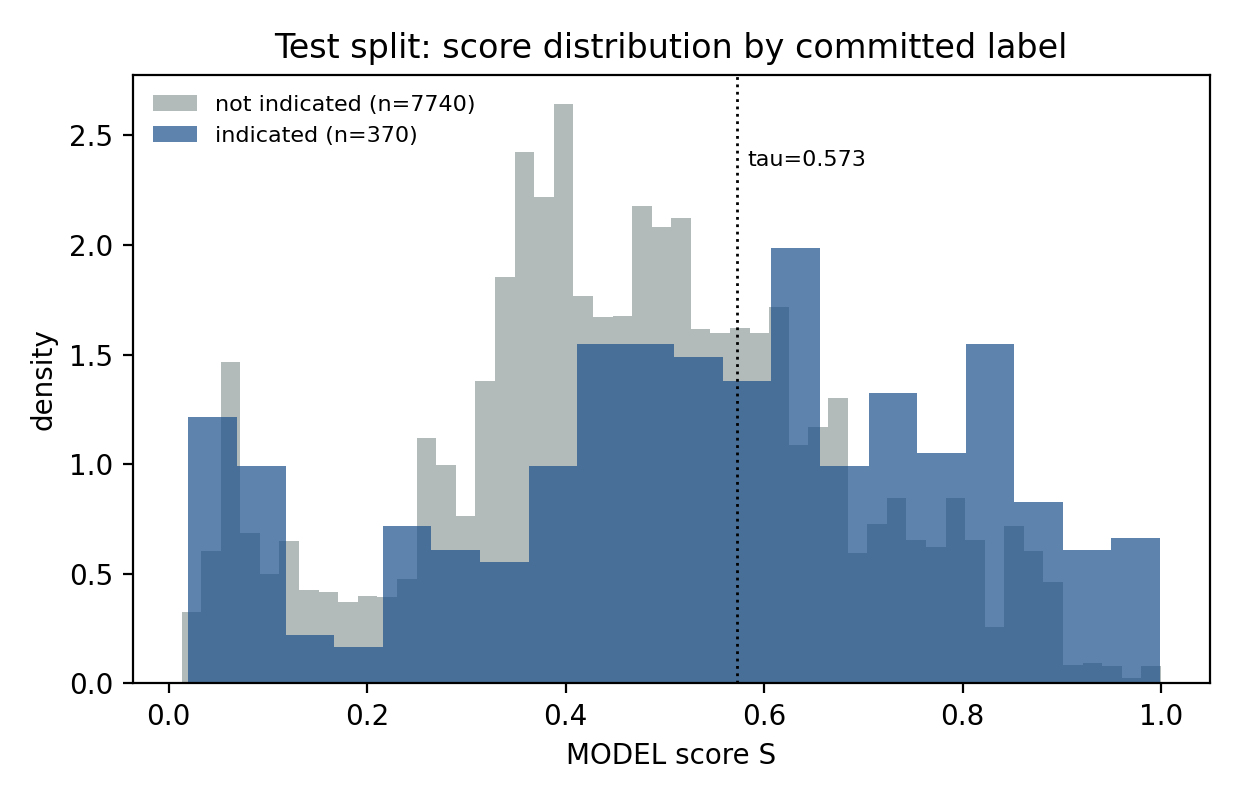
\includegraphics[width=0.72\textwidth]{figures/fig_score_dist.png}
\caption{Test-split score distributions by committed label. The classes separate but overlap -- the honest picture behind the AUPRC numbers; $\tau$ sits at the calibration optimum, not at a visual valley.}\end{figure}
\begin{figure}[h]\centering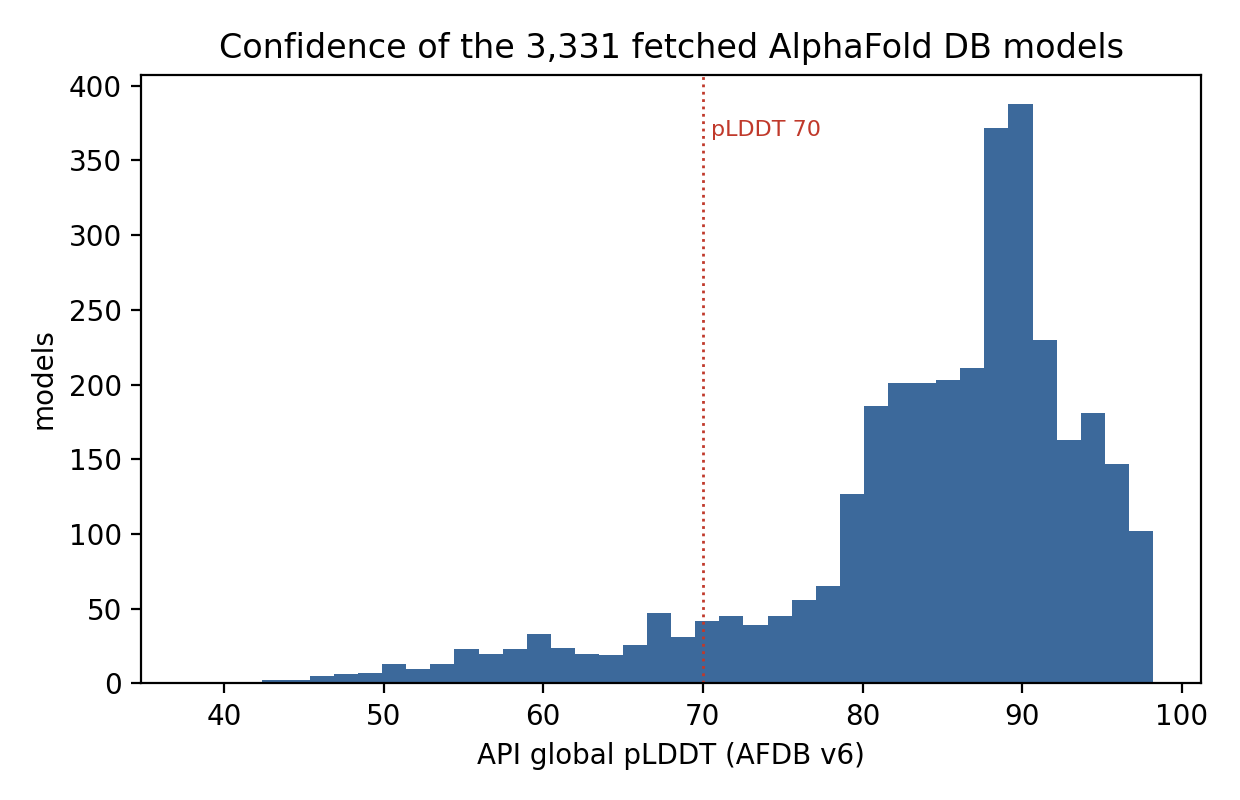
\includegraphics[width=0.72\textwidth]{figures/fig_plddt.png}
\caption{Structure confidence across the fetched model set: mean global pLDDT 84.3, 89.9\% of models at pLDDT $\geq 70$, 0.8\% below 50. Structural comparisons in this slice rest almost entirely on high-confidence models.}\end{figure}

\subsection{Per-species detail (test split)}
\begin{longtable}{l r r r r}
\caption{Held-out test species: panel size, true indicated products, product recovery and inventory coverage at frozen $\tau=0.5727$. One of the 21 test species had no scorable (toxin, product) pair (no indicated reference passed the prefilter) and is omitted here -- recorded as a negative.}\\
\hline\hline species & toxins & products & recovery & inv.\ covered \\ \hline\hline \endfirsthead
\hline\hline species & toxins & products & recovery & inv.\ covered \\ \hline\hline \endhead
\textit{Acanthophis spp} & 15 & 2 & 0.50 & 0.47 \\
\textit{Bitis gabonica} & 9 & 2 & 0.50 & 0.44 \\
\textit{Bothriechis schlegelii} & 3 & 1 & 1.00 & 1.00 \\
\textit{Bothrops mattogrossensis} & 5 & 2 & 0.00 & 0.40 \\
\textit{Bungarus fasciatus} & 13 & 3 & 0.33 & 0.54 \\
\textit{Crotalus atrox} & 44 & 2 & 1.00 & 0.75 \\
\textit{Crotalus horridus} & 45 & 1 & 1.00 & 0.89 \\
\textit{Crotalus molossus} & 9 & 2 & 1.00 & 0.78 \\
\textit{Crotalus viridis} & 20 & 2 & 1.00 & 0.70 \\
\textit{Daboia russelii} & 40 & 4 & 1.00 & 0.78 \\
\textit{Dendroaspis jamesoni} & 9 & 2 & 1.00 & 0.56 \\
\textit{Gloydius halys} & 28 & 1 & 0.00 & 0.61 \\
\textit{Gloydius ussuriensis} & 12 & 1 & 1.00 & 0.92 \\
\textit{Naja annulifera} & 18 & 1 & 1.00 & 0.94 \\
\textit{Naja melanoleuca} & 8 & 2 & 1.00 & 0.75 \\
\textit{Naja samarensis} & 1 & 1 & 1.00 & 1.00 \\
\textit{Naja sputatrix} & 31 & 1 & 0.00 & 0.81 \\
\textit{Ophiophagus hannah} & 118 & 2 & 0.50 & 0.25 \\
\textit{Porthidium ophryomegas} & 1 & 1 & 0.00 & 0.00 \\
\textit{Vipera ursinii} & 1 & 1 & 0.00 & 1.00 \\
\hline\hline\end{longtable}

\subsection{Per-species detail (target set)}
\begin{longtable}{l l r r r}
\caption{Target set: all 38 CRITICAL/HIGH species with toxin records. Toxins = in-panel toxins; model / baseline = toxins inferred-covered by the cascade at $\tau$ and by the committed heuristic at T=80.}\\
\hline\hline species & gap class & toxins & model & baseline \\ \hline\hline \endfirsthead
\hline\hline species & gap class & toxins & model & baseline \\ \hline\hline \endhead
\textit{Atheris chlorechis} & HIGH & 1 & 1 & 1 \\
\textit{Atheris squamigera} & HIGH & 1 & 1 & 1 \\
\textit{Atractaspis andersonii} & CRITICAL & 2 & 0 & 0 \\
\textit{Atractaspis bibronii} & HIGH & 1 & 0 & 0 \\
\textit{Atractaspis engaddensis} & HIGH & 3 & 0 & 0 \\
\textit{Atractaspis irregularis} & HIGH & 2 & 0 & 0 \\
\textit{Atropoides spp} & HIGH & 2 & 2 & 2 \\
\textit{Bitis nasicornis} & HIGH & 3 & 1 & 1 \\
\textit{Bitis rhinoceros} & HIGH & 10 & 3 & 2 \\
\textit{Bothriechis spp} & HIGH & 1 & 1 & 1 \\
\textit{Bothrops bilineatus} & CRITICAL & 1 & 1 & 1 \\
\textit{Bothrops leucurus} & CRITICAL & 10 & 6 & 5 \\
\textit{Bungarus flaviceps} & HIGH & 22 & 6 & 6 \\
\textit{Calliophis bivirgatus} & HIGH & 22 & 11 & 11 \\
\textit{Cerrophidion sasai} & HIGH & 1 & 1 & 1 \\
\textit{Crotalus ruber} & HIGH & 3 & 2 & 1 \\
\textit{Crotalus tzabcan} & HIGH & 8 & 7 & 8 \\
\textit{Daboia palaestinae} & CRITICAL & 7 & 2 & 5 \\
\textit{Eristocophis macmahoni} & HIGH & 6 & 1 & 2 \\
\textit{Gloydius tsushimaensis} & HIGH & 1 & 1 & 1 \\
\textit{Micrurus lemniscatus} & HIGH & 1 & 0 & 0 \\
\textit{Micrurus mipartitus} & HIGH & 15 & 7 & 8 \\
\textit{Micrurus surinamensis} & HIGH & 6 & 0 & 0 \\
\textit{Naja anchietae} & CRITICAL & 1 & 1 & 1 \\
\textit{Naja annulata} & HIGH & 2 & 2 & 1 \\
\textit{Naja christyi} & HIGH & 1 & 1 & 1 \\
\textit{Naja pallida} & HIGH & 3 & 3 & 3 \\
\textit{Naja sagittifera} & CRITICAL & 2 & 1 & 1 \\
\textit{Proatheris superciliaris} & HIGH & 2 & 0 & 0 \\
\textit{Protobothrops elegans} & HIGH & 23 & 12 & 15 \\
\textit{Protobothrops jerdonii} & HIGH & 19 & 18 & 17 \\
\textit{Protobothrops mangshanensis} & HIGH & 2 & 1 & 1 \\
\textit{Pseudocerastes fieldi} & HIGH & 3 & 1 & 2 \\
\textit{Trimeresurus albolabris} & HIGH & 18 & 12 & 9 \\
\textit{Trimeresurus purpureomaculatus} & HIGH & 5 & 1 & 1 \\
\textit{Trimeresurus stejnegeri} & HIGH & 68 & 47 & 44 \\
\textit{Vipera nikolskii} & HIGH & 5 & 4 & 5 \\
\textit{Vipera renardi} & HIGH & 7 & 4 & 3 \\
\hline\hline\end{longtable}

\begin{table}[h]\centering\small
\caption{Pipeline statistics (all artifacts committed; every count regenerable from \texttt{modeling/code/}).}
\begin{tabular}{l r}\hline\hline
quantity & value \\ \hline\hline
panel queries (all in-scope toxins with sequences) & 3,644 \\
\quad of which target (CRITICAL/HIGH) & 290 \\
scored (toxin, product) rows & 62475 \\
unique shortlisted (toxin, reference) pairs & 78468 \\
\quad structure-scored (status ok) & 64470 \\
\quad sequence-only fallback (no structure) & 10180 \\
\quad fallback (alignment $<$ 8 positions) & 3812 \\
AFDB v6 models fetched (100\%% success) & 3331 \\
\quad models with usable C$\alpha$ trace & 3,059 \\
calibration / test species & 85 / 21 \\
calibration / test (toxin, product) pairs & 48,317 / 8,110 \\
\hline\hline\end{tabular}\end{table}

\section{Discussion and limitations}
The result is a real but modest win, stated precisely: under a species-level holdout that mirrors the actual use case (a new or uncovered species arrives; which existing products plausibly cover its toxins?), structural re-scoring of sequence shortlists improves pair ranking over the established heuristic, with a bootstrap CI that excludes zero under the pre-registered criterion. On the target set the two methods largely agree, which is itself the scientifically useful finding: the heuristic's headline coverage estimate (about half the gap inventory plausibly covered) survives scrutiny by a stronger method, while the model re-ranks \emph{which} products to trust per toxin.

Limitations bound every claim. The labels are manufacturer/regulatory \emph{indications}, not binding measurements; pair-level precision is capped by label coarseness. AlphaFold models are predictions, and 261 panel accessions have none. The epitope term is a solvent-exposure and chemistry-class proxy, not a paratope--epitope simulation; polyclonal avidity, glycosylation, and neutralization (as opposed to binding) are all outside the model. The weight triple was fixed a priori for honesty, not optimized; a fitted model would likely score higher and prove less. And per the access-only gate, nothing here spent money, created accounts, or communicated as anyone.

\section{Reproducibility}
Every number in this paper regenerates from \texttt{modeling/code/} in eight steps: \texttt{panel.py} (panel + seeded split) $\rightarrow$ \texttt{baseline\_check.py} (baseline equivalence) $\rightarrow$ \texttt{shortlist.py} (sequence stage) $\rightarrow$ \texttt{fetch\_afdb.py} (structure acquisition) $\rightarrow$ \texttt{features.py} (structural features) $\rightarrow$ \texttt{score.py} (assembly, calibration, evaluation) $\rightarrow$ \texttt{target\_coverage.py} (target set) $\rightarrow$ \texttt{figures.py}. Each step reads only committed inputs or earlier committed outputs against the committed B09 inputs and the sha256-locked AFDB fetch manifest. The gate file, split assignment, fetch manifest, score tables, and this paper's sources are byte-locked in \texttt{modeling/manifests/slice-manifest.md}; the model PDB files (577\,MB) are hash-locked and regenerable from their recorded URLs rather than committed, by size. Commit order -- gates, design, results, seal -- is the lock-order proof.

\begin{thebibliography}{9}\small
\bibitem{who-factsheet} WHO. Snakebite envenoming (fact sheet). \url{https://www.who.int/news-room/fact-sheets/detail/snakebite-envenoming}
\bibitem{who-trs1004} WHO. Guidelines for the production, control and regulation of snake antivenom immunoglobulins, TRS 1004 Annex 5 (2017). \url{https://cdn.who.int/media/docs/default-source/biologicals/blood-products/document-migration/antivenomglrevwho_trs_1004_web_annex_5.pdf}
\bibitem{longbottom2018} Longbottom J, et al. Vulnerability to snakebite envenoming: a global mapping of hotspots. \emph{The Lancet} (2018). \url{https://pmc.ncbi.nlm.nih.gov/articles/PMC6115328/}; data/code: \url{https://github.com/joshlongbottom/snakebite}
\bibitem{uniprot} The UniProt Consortium. UniProtKB, query \texttt{keyword:KW-0800 AND taxonomy\_id:8570}, retrieved 2026-09-23 (committed raw responses).
\bibitem{afdb2024} Varadi M, et al. AlphaFold Protein Structure Database in 2024. \emph{Nucleic Acids Research} 52(D1):D368. \url{https://academic.oup.com/nar/article/52/D1/D368/7337620}
\bibitem{gutierrez2009} Guti\'errez JM, et al. Snake venomics and antivenomics: Proteomic tools in the design and control of antivenoms. \emph{J.\ Proteomics} (2009). \url{https://pubmed.ncbi.nlm.nih.gov/19344652/}
\bibitem{gutierrez2010} Guti\'errez JM, et al. Antivenomics and venom phenotyping. \emph{J.\ Proteomics} (2010). \url{https://pubmed.ncbi.nlm.nih.gov/20036274/}
\bibitem{tmscore2004} Zhang Y, Skolnick J. Scoring function for automated assessment of protein structure template quality. \emph{Proteins} 57:702--710 (2004). \url{https://pubmed.ncbi.nlm.nih.gov/15476259/}
\bibitem{edlib} \v{S}o\v{s}i\'c M, \v{S}iki\'c M. Edlib: a C/C++ library for fast, exact sequence alignment using edit distance. \emph{Bioinformatics} 33(9):1394 (2017). \url{https://academic.oup.com/bioinformatics/article/33/9/1394/2964763}
\end{thebibliography}
\end{document}
